% Options for packages loaded elsewhere
\PassOptionsToPackage{unicode}{hyperref}
\PassOptionsToPackage{hyphens}{url}
\PassOptionsToPackage{dvipsnames,svgnames,x11names}{xcolor}
%
\documentclass[
  8pt,
  ignorenonframetext,
]{beamer}
\title{Programmation sous R\\
Chapitre 1: Initiation au logiciel R}
\author{Mohamed Essaied Hamrita\\
\href{mailto:mhamrita@gmail.com}{\nolinkurl{mhamrita@gmail.com}}\\
\href{https:github.com/Hamrita}{github.com/Hamrita}}
\date{2023-2024}
\institute{Université de Sousse - Tunisie}

\usepackage{pgfpages}
\setbeamertemplate{caption}[numbered]
\setbeamertemplate{caption label separator}{: }
\setbeamercolor{caption name}{fg=normal text.fg}
\beamertemplatenavigationsymbolsempty
% Prevent slide breaks in the middle of a paragraph
\widowpenalties 1 10000
\raggedbottom
\setbeamertemplate{part page}{
  \centering
  \begin{beamercolorbox}[sep=16pt,center]{part title}
    \usebeamerfont{part title}\insertpart\par
  \end{beamercolorbox}
}
\setbeamertemplate{section page}{
  \centering
  \begin{beamercolorbox}[sep=12pt,center]{part title}
    \usebeamerfont{section title}\insertsection\par
  \end{beamercolorbox}
}
\setbeamertemplate{subsection page}{
  \centering
  \begin{beamercolorbox}[sep=8pt,center]{part title}
    \usebeamerfont{subsection title}\insertsubsection\par
  \end{beamercolorbox}
}
\AtBeginPart{
  \frame{\partpage}
}
\AtBeginSection{
  \ifbibliography
  \else
    \frame{\sectionpage}
  \fi
}
\AtBeginSubsection{
  \frame{\subsectionpage}
}
\usepackage{amsmath,amssymb}
\usepackage{lmodern}
\usepackage{iftex}
\ifPDFTeX
  \usepackage[T1]{fontenc}
  \usepackage[utf8]{inputenc}
  \usepackage{textcomp} % provide euro and other symbols
\else % if luatex or xetex
  \usepackage{unicode-math}
  \defaultfontfeatures{Scale=MatchLowercase}
  \defaultfontfeatures[\rmfamily]{Ligatures=TeX,Scale=1}
\fi
\usetheme[]{Frankfurt}
\usecolortheme{dolphin}
\usefonttheme{professionalfonts}
% Use upquote if available, for straight quotes in verbatim environments
\IfFileExists{upquote.sty}{\usepackage{upquote}}{}
\IfFileExists{microtype.sty}{% use microtype if available
  \usepackage[]{microtype}
  \UseMicrotypeSet[protrusion]{basicmath} % disable protrusion for tt fonts
}{}
\makeatletter
\@ifundefined{KOMAClassName}{% if non-KOMA class
  \IfFileExists{parskip.sty}{%
    \usepackage{parskip}
  }{% else
    \setlength{\parindent}{0pt}
    \setlength{\parskip}{6pt plus 2pt minus 1pt}}
}{% if KOMA class
  \KOMAoptions{parskip=half}}
\makeatother
\usepackage{xcolor}
\IfFileExists{xurl.sty}{\usepackage{xurl}}{} % add URL line breaks if available
\IfFileExists{bookmark.sty}{\usepackage{bookmark}}{\usepackage{hyperref}}
\hypersetup{
  colorlinks=true,
  linkcolor={Maroon},
  filecolor={Maroon},
  citecolor={Blue},
  urlcolor={blue},
  pdfcreator={LaTeX via pandoc}}
\urlstyle{same} % disable monospaced font for URLs
\newif\ifbibliography
\usepackage{color}
\usepackage{fancyvrb}
\newcommand{\VerbBar}{|}
\newcommand{\VERB}{\Verb[commandchars=\\\{\}]}
\DefineVerbatimEnvironment{Highlighting}{Verbatim}{commandchars=\\\{\}}
% Add ',fontsize=\small' for more characters per line
\usepackage{framed}
\definecolor{shadecolor}{RGB}{248,248,248}
\newenvironment{Shaded}{\begin{snugshade}}{\end{snugshade}}
\newcommand{\AlertTok}[1]{\textcolor[rgb]{0.94,0.16,0.16}{#1}}
\newcommand{\AnnotationTok}[1]{\textcolor[rgb]{0.56,0.35,0.01}{\textbf{\textit{#1}}}}
\newcommand{\AttributeTok}[1]{\textcolor[rgb]{0.77,0.63,0.00}{#1}}
\newcommand{\BaseNTok}[1]{\textcolor[rgb]{0.00,0.00,0.81}{#1}}
\newcommand{\BuiltInTok}[1]{#1}
\newcommand{\CharTok}[1]{\textcolor[rgb]{0.31,0.60,0.02}{#1}}
\newcommand{\CommentTok}[1]{\textcolor[rgb]{0.56,0.35,0.01}{\textit{#1}}}
\newcommand{\CommentVarTok}[1]{\textcolor[rgb]{0.56,0.35,0.01}{\textbf{\textit{#1}}}}
\newcommand{\ConstantTok}[1]{\textcolor[rgb]{0.00,0.00,0.00}{#1}}
\newcommand{\ControlFlowTok}[1]{\textcolor[rgb]{0.13,0.29,0.53}{\textbf{#1}}}
\newcommand{\DataTypeTok}[1]{\textcolor[rgb]{0.13,0.29,0.53}{#1}}
\newcommand{\DecValTok}[1]{\textcolor[rgb]{0.00,0.00,0.81}{#1}}
\newcommand{\DocumentationTok}[1]{\textcolor[rgb]{0.56,0.35,0.01}{\textbf{\textit{#1}}}}
\newcommand{\ErrorTok}[1]{\textcolor[rgb]{0.64,0.00,0.00}{\textbf{#1}}}
\newcommand{\ExtensionTok}[1]{#1}
\newcommand{\FloatTok}[1]{\textcolor[rgb]{0.00,0.00,0.81}{#1}}
\newcommand{\FunctionTok}[1]{\textcolor[rgb]{0.00,0.00,0.00}{#1}}
\newcommand{\ImportTok}[1]{#1}
\newcommand{\InformationTok}[1]{\textcolor[rgb]{0.56,0.35,0.01}{\textbf{\textit{#1}}}}
\newcommand{\KeywordTok}[1]{\textcolor[rgb]{0.13,0.29,0.53}{\textbf{#1}}}
\newcommand{\NormalTok}[1]{#1}
\newcommand{\OperatorTok}[1]{\textcolor[rgb]{0.81,0.36,0.00}{\textbf{#1}}}
\newcommand{\OtherTok}[1]{\textcolor[rgb]{0.56,0.35,0.01}{#1}}
\newcommand{\PreprocessorTok}[1]{\textcolor[rgb]{0.56,0.35,0.01}{\textit{#1}}}
\newcommand{\RegionMarkerTok}[1]{#1}
\newcommand{\SpecialCharTok}[1]{\textcolor[rgb]{0.00,0.00,0.00}{#1}}
\newcommand{\SpecialStringTok}[1]{\textcolor[rgb]{0.31,0.60,0.02}{#1}}
\newcommand{\StringTok}[1]{\textcolor[rgb]{0.31,0.60,0.02}{#1}}
\newcommand{\VariableTok}[1]{\textcolor[rgb]{0.00,0.00,0.00}{#1}}
\newcommand{\VerbatimStringTok}[1]{\textcolor[rgb]{0.31,0.60,0.02}{#1}}
\newcommand{\WarningTok}[1]{\textcolor[rgb]{0.56,0.35,0.01}{\textbf{\textit{#1}}}}
\setlength{\emergencystretch}{3em} % prevent overfull lines
\providecommand{\tightlist}{%
  \setlength{\itemsep}{0pt}\setlength{\parskip}{0pt}}
\setcounter{secnumdepth}{-\maxdimen} % remove section numbering
\setbeamertemplate{navigation symbols}{}
\setbeamertemplate{footline}[page number]
\ifLuaTeX
  \usepackage{selnolig}  % disable illegal ligatures
\fi

\begin{document}
\frame{\titlepage}

\begin{frame}[allowframebreaks]
  \tableofcontents[hideallsubsections]
\end{frame}
\hypertarget{introduction}{%
\section{Introduction}\label{introduction}}

\begin{frame}{Introduction}
R est un logiciel de calcul scientifique interactif \textbf{libre} et
\textbf{gratuit} qui possède une large collection d'outils statistiques
et graphiques. Plusieurs sites sont consacrés à ce logiciel. Parmi
lesquels, je cite:

\begin{itemize}
\item
  \url{http://http://www.r-project.org/}. Le site officiel du logiciel
  dans lequel on trouve une description exhaustive sur le langage R et
  fournit les liens indispensables pour les différents téléchargements.
\item
  \url{http://www.statmethods.net/}. QuickR, un site dans lequel on
  trouve les fonctions les plus utiles lors d'une analyse statistique
  uni et multi-variée.
\item
  \url{https://www.learnbyexample.org/r/} Apprendre R par des exemples.
\end{itemize}
\end{frame}

\begin{frame}{Installation du logiciel R}
\protect\hypertarget{installation-du-logiciel-r}{}
Dans la page de r-project, on trouve des versions de R compilée et sont
disponibles pour Windows, Linux et Mac OS X. Ici, on décrit
l'installation de R sous Windows. Tout d'abord, on se rendre sur cette
page: \url{http://cran.r-project.org/bin/windows/base/} et l'on suivra
le premier lien pour télécharger le programme d'installation. \pause

\begin{center}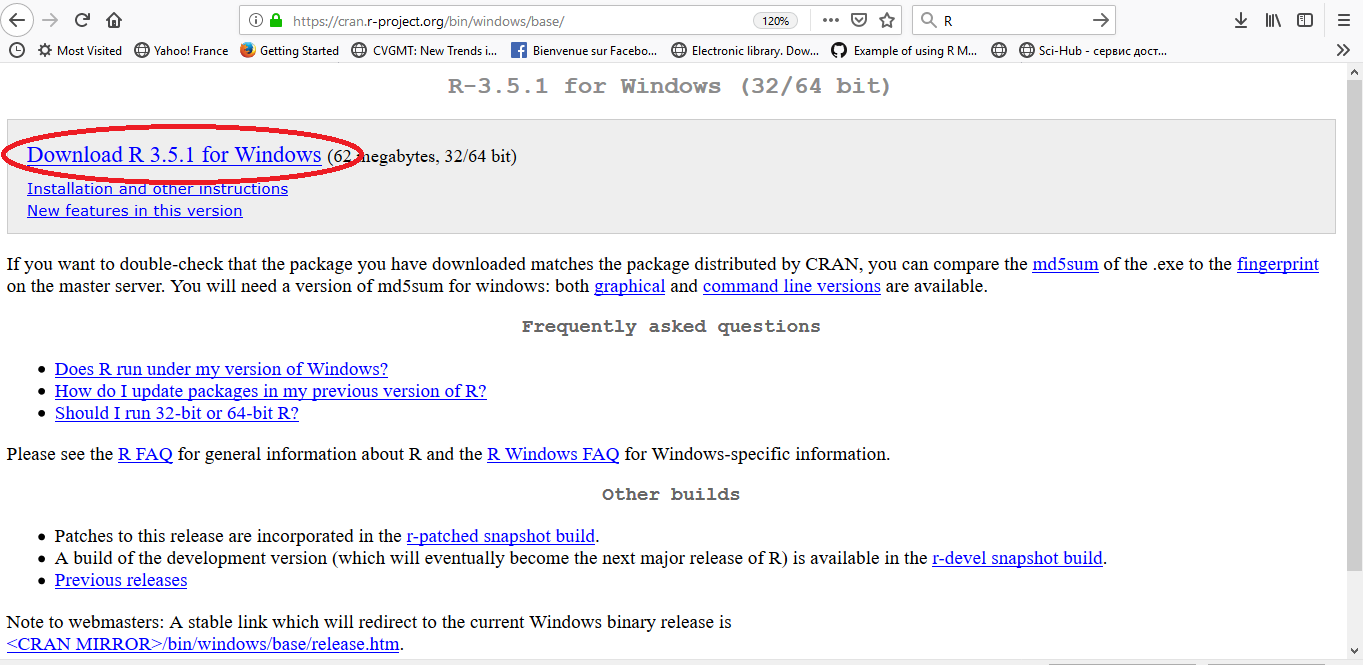
\includegraphics[width=0.8\linewidth,height=0.5\textheight]{fig1} \end{center}

\pause

Une fois le programme d'installation lancé, il suffira d'installer R
avec les options par défaut.
\end{frame}

\begin{frame}{Installation de RStudio}
\protect\hypertarget{installation-de-rstudio}{}
Une fois R est correctement installé, je vous recommande fortement
d'installer RStudio qui est téléchargeable depuis
\url{http://www.rstudio.com/products/rstudio/download/}:

\pause

\begin{center}
\includegraphics[width=0.8\linewidth,height=0.7\textheight]{fig2} \end{center}
\end{frame}

\begin{frame}{Mise à jour de R}
\protect\hypertarget{mise-uxe0-jour-de-r}{}
Pour mettre à jour R sous Windows, il suffit de télécharger et installer
la dernière version du programme d'installation.

Il est à remarquer que la nouvelle version sera installée à côté de
l'ancienne version. Afin de libérer de l'espace, vous pouvez
désinstaller l'ancienne version en utilisant l'utilitaire
\textbf{\emph{désinstaller un programme}} de Windows.

Lorsque plusieurs versions de R sont disponibles, RStudio choisit par
défaut la plus récente.
\end{frame}

\hypertarget{duxe9marrer-avec-r}{%
\section{Démarrer avec R}\label{duxe9marrer-avec-r}}

\begin{frame}[fragile]{Le répartoire courant}
\protect\hypertarget{le-ruxe9partoire-courant}{}
Pour pouvoir récupérer des données, il est utile de connaître le
répertoire de travail, c'est-à-dire le répertoire sous lequel les divers
résultats seront sauvegardés par défaut. Ce dernier s'obtient à l'aide
la commande :

\begin{Shaded}
\begin{Highlighting}[]
\FunctionTok{getwd}\NormalTok{()}
\end{Highlighting}
\end{Shaded}

\begin{verbatim}
[1] "D:/Enseignement/R/Diapos_2023/R/Chap1"
\end{verbatim}

Tandis que la commande

\begin{Shaded}
\begin{Highlighting}[]
\FunctionTok{setwd}\NormalTok{(}\StringTok{"C:/User/Mes documents/CoursR"}\NormalTok{)}
\end{Highlighting}
\end{Shaded}

change de répertoire courant.
\end{frame}

\begin{frame}[fragile]{Démarrer avec R}
\protect\hypertarget{duxe9marrer-avec-r-1}{}
\begin{Shaded}
\begin{Highlighting}[]
\CommentTok{\# ceci est un commentaire}

\CommentTok{\# opérateurs: +, {-}, *, \^{} (**), \%/\%, \%\%}

\CommentTok{\# opérations matricielles: \%*\%, solve(), as.vector(),}
\CommentTok{\# det(), t()}
\DecValTok{5}\SpecialCharTok{\%/\%}\DecValTok{3}
\end{Highlighting}
\end{Shaded}

\begin{verbatim}
[1] 1
\end{verbatim}

\begin{Shaded}
\begin{Highlighting}[]
\FunctionTok{cos}\NormalTok{(pi}\SpecialCharTok{/}\DecValTok{3}\NormalTok{)}
\end{Highlighting}
\end{Shaded}

\begin{verbatim}
[1] 0.5
\end{verbatim}

\begin{Shaded}
\begin{Highlighting}[]
\DocumentationTok{\#\# Saisie des données}
\NormalTok{XX }\OtherTok{\textless{}{-}} \FunctionTok{c}\NormalTok{(}\StringTok{"M"}\NormalTok{, }\StringTok{"M"}\NormalTok{, }\StringTok{"D"}\NormalTok{, }\StringTok{"C"}\NormalTok{, }\StringTok{"C"}\NormalTok{, }\StringTok{"M"}\NormalTok{, }\FunctionTok{rep}\NormalTok{(}\StringTok{"C"}\NormalTok{, }\DecValTok{3}\NormalTok{), }\StringTok{"M"}\NormalTok{, }\StringTok{"C"}\NormalTok{,}
    \StringTok{"M"}\NormalTok{, }\StringTok{"V"}\NormalTok{, }\StringTok{"M"}\NormalTok{, }\StringTok{"V"}\NormalTok{, }\StringTok{"D"}\NormalTok{, }\FunctionTok{rep}\NormalTok{(}\StringTok{"C"}\NormalTok{, }\DecValTok{3}\NormalTok{), }\StringTok{"M"}\NormalTok{)}
\end{Highlighting}
\end{Shaded}
\end{frame}

\begin{frame}[fragile]
\begin{Shaded}
\begin{Highlighting}[]
\CommentTok{\# Créer un objet x en lui affectant le nombre 2}
\NormalTok{x }\OtherTok{\textless{}{-}} \DecValTok{2}
\NormalTok{nom }\OtherTok{\textless{}{-}} \StringTok{"Mohamed"}
\CommentTok{\# Créer un objet x et afficher son contenu}
\NormalTok{(x }\OtherTok{\textless{}{-}} \DecValTok{2}\NormalTok{)}
\end{Highlighting}
\end{Shaded}

\begin{verbatim}
[1] 2
\end{verbatim}

Le logiciel R travail avec des objets. Mais quelle est la classe de ces
objets? de quels modes?
\end{frame}

\hypertarget{les-diffuxe9rents-objets}{%
\section{Les différents objets}\label{les-diffuxe9rents-objets}}

\begin{frame}[fragile]{Les différents objets}
Les différents objets de R sont: vecteur, matrice, liste, tableau des
données ou ts (time series).

\begin{itemize}
\tightlist
\item
  Vecteur: un vecteur peut être de mode numérique, caractère, complexe
  ou logique.
\end{itemize}

\begin{Shaded}
\begin{Highlighting}[]
\NormalTok{x1}\OtherTok{\textless{}{-}}\FunctionTok{c}\NormalTok{(}\DecValTok{1}\NormalTok{,}\SpecialCharTok{{-}}\DecValTok{5}\NormalTok{)  }\CommentTok{\# vecteur numérique}
\FunctionTok{mode}\NormalTok{(x1)     }\CommentTok{\# afficher le mode de l\textquotesingle{}objet x1.}
\end{Highlighting}
\end{Shaded}

\begin{verbatim}
[1] "numeric"
\end{verbatim}

\begin{Shaded}
\begin{Highlighting}[]
\NormalTok{x2}\OtherTok{\textless{}{-}}\FunctionTok{c}\NormalTok{(}\StringTok{"Mohamed"}\NormalTok{,}\StringTok{"Sarah"}\NormalTok{)  }\CommentTok{\# vecteur caractère}
\NormalTok{x3}\OtherTok{\textless{}{-}}\FunctionTok{c}\NormalTok{(1i,}\DecValTok{1}\SpecialCharTok{{-}}\NormalTok{1i,}\SpecialCharTok{{-}}\DecValTok{2}\SpecialCharTok{+}\NormalTok{3i) }\CommentTok{\# vecteur complexe}
\NormalTok{x4}\OtherTok{\textless{}{-}}\FunctionTok{c}\NormalTok{(}\ConstantTok{TRUE}\NormalTok{,}\ConstantTok{FALSE}\NormalTok{,T,F)  }\CommentTok{\# vecteur logique}
\end{Highlighting}
\end{Shaded}

Pour créer des séries régulières, on peut utiliser les fonctions
suivantes:

\begin{Shaded}
\begin{Highlighting}[]
\CommentTok{\# c(), seq(), : ou rep()}
\end{Highlighting}
\end{Shaded}
\end{frame}

\begin{frame}[fragile]
\textbf{La fonction c()}

Pour avoir l'aide de cette fonction, tapez ?c

\begin{Shaded}
\begin{Highlighting}[]
\NormalTok{x1}\OtherTok{\textless{}{-}}\FunctionTok{c}\NormalTok{(}\DecValTok{1}\NormalTok{,}\DecValTok{0}\NormalTok{,}\DecValTok{5}\NormalTok{,}\SpecialCharTok{{-}}\DecValTok{4}\NormalTok{)  }\CommentTok{\# création d\textquotesingle{}un vecteur}
\NormalTok{x1[}\DecValTok{3}\NormalTok{]            }\CommentTok{\# extraction du troisième élément de x1}
\end{Highlighting}
\end{Shaded}

\begin{verbatim}
[1] 5
\end{verbatim}

\begin{Shaded}
\begin{Highlighting}[]
\NormalTok{x1[}\SpecialCharTok{{-}}\DecValTok{1}\NormalTok{]           }\CommentTok{\# afficher tous les éléments de x1 sauf le premier}
\end{Highlighting}
\end{Shaded}

\begin{verbatim}
[1]  0  5 -4
\end{verbatim}

\begin{Shaded}
\begin{Highlighting}[]
\NormalTok{x1[x1}\SpecialCharTok{\textgreater{}}\DecValTok{2}\NormalTok{]         }\CommentTok{\# extraire les éléments supèrieur à 2.}
\end{Highlighting}
\end{Shaded}

\begin{verbatim}
[1] 5
\end{verbatim}

\begin{Shaded}
\begin{Highlighting}[]
\NormalTok{x1}\SpecialCharTok{\textgreater{}}\DecValTok{2}             \CommentTok{\# vecteur logique pour tester si x1\textgreater{}2 ou non.}
\end{Highlighting}
\end{Shaded}

\begin{verbatim}
[1] FALSE FALSE  TRUE FALSE
\end{verbatim}

\begin{Shaded}
\begin{Highlighting}[]
\NormalTok{x11}\OtherTok{\textless{}{-}}\FunctionTok{c}\NormalTok{(}\StringTok{"a"}\NormalTok{,}\StringTok{"A"}\NormalTok{,}\StringTok{"b"}\NormalTok{,}\StringTok{"B"}\NormalTok{)}
\NormalTok{lettres15}\OtherTok{\textless{}{-}}\NormalTok{letters[}\FunctionTok{c}\NormalTok{(}\DecValTok{1}\NormalTok{,}\DecValTok{5}\NormalTok{)] }\CommentTok{\# création d\textquotesingle{}un vecteur contenant la }
\CommentTok{\# première et la cinquième lettres minuscules}
\NormalTok{lettres15}
\end{Highlighting}
\end{Shaded}

\begin{verbatim}
[1] "a" "e"
\end{verbatim}

\begin{Shaded}
\begin{Highlighting}[]
\NormalTok{LETTRES15}\OtherTok{\textless{}{-}}\NormalTok{LETTERS[}\FunctionTok{c}\NormalTok{(}\DecValTok{1}\NormalTok{,}\DecValTok{5}\NormalTok{)]  }\CommentTok{\# idem mais majuscules}
\NormalTok{LETTRES15}
\end{Highlighting}
\end{Shaded}

\begin{verbatim}
[1] "A" "E"
\end{verbatim}
\end{frame}

\begin{frame}[fragile]
\textbf{La fonction \texttt{seq()}}

la fonction \texttt{seq()} est utilisée pour créer des séquences.

\begin{Shaded}
\begin{Highlighting}[]
\NormalTok{seq1}\OtherTok{\textless{}{-}}\FunctionTok{seq}\NormalTok{(}\DecValTok{0}\NormalTok{,}\DecValTok{1}\NormalTok{,}\AttributeTok{by=}\FloatTok{0.1}\NormalTok{)  }\CommentTok{\# séquence de 0 à 1 par incrémentation 0.1.}
\NormalTok{seq1}
\end{Highlighting}
\end{Shaded}

\begin{verbatim}
 [1] 0.0 0.1 0.2 0.3 0.4 0.5 0.6 0.7 0.8 0.9 1.0
\end{verbatim}

\begin{Shaded}
\begin{Highlighting}[]
\FunctionTok{length}\NormalTok{(seq1)   }\CommentTok{\# afficher la longueur de seq1}
\end{Highlighting}
\end{Shaded}

\begin{verbatim}
[1] 11
\end{verbatim}

\begin{Shaded}
\begin{Highlighting}[]
\NormalTok{seq2}\OtherTok{\textless{}{-}}\FunctionTok{seq}\NormalTok{(}\DecValTok{0}\NormalTok{,}\DecValTok{1}\NormalTok{,}\AttributeTok{len=}\DecValTok{5}\NormalTok{)   }\CommentTok{\# séquence de 0 à 1 de longueur 5.}
\NormalTok{seq2}
\end{Highlighting}
\end{Shaded}

\begin{verbatim}
[1] 0.00 0.25 0.50 0.75 1.00
\end{verbatim}

\begin{Shaded}
\begin{Highlighting}[]
\NormalTok{seq3}\OtherTok{\textless{}{-}}\FunctionTok{seq}\NormalTok{(}\DecValTok{0}\NormalTok{,}\DecValTok{1}\NormalTok{,}\AttributeTok{len=}\DecValTok{11}\NormalTok{)  }\CommentTok{\# même résultat que seq1}
\NormalTok{seq3}
\end{Highlighting}
\end{Shaded}

\begin{verbatim}
 [1] 0.0 0.1 0.2 0.3 0.4 0.5 0.6 0.7 0.8 0.9 1.0
\end{verbatim}
\end{frame}

\begin{frame}[fragile]{}
\protect\hypertarget{section}{}
\textbf{Les fonctions : et rep()}

la fonction \texttt{:} est utilisée pour créer des séquences entière de
a à b.

\begin{Shaded}
\begin{Highlighting}[]
\NormalTok{seq}\OtherTok{\textless{}{-}}\DecValTok{1}\SpecialCharTok{:}\DecValTok{5}  \CommentTok{\# séquence entière de 1 à 5.}
\NormalTok{seq}
\end{Highlighting}
\end{Shaded}

\begin{verbatim}
[1] 1 2 3 4 5
\end{verbatim}

\begin{Shaded}
\begin{Highlighting}[]
\NormalTok{seqi}\OtherTok{\textless{}{-}}\DecValTok{6}\SpecialCharTok{:{-}}\DecValTok{4}
\NormalTok{seqi}
\end{Highlighting}
\end{Shaded}

\begin{verbatim}
 [1]  6  5  4  3  2  1  0 -1 -2 -3 -4
\end{verbatim}

La fonction \texttt{rep()} est utilisée lorsqu'on veut répéter un
élément ou un vecteur n fois.

\begin{Shaded}
\begin{Highlighting}[]
\FunctionTok{rep}\NormalTok{(}\DecValTok{1}\NormalTok{,}\DecValTok{5}\NormalTok{)}
\end{Highlighting}
\end{Shaded}

\begin{verbatim}
[1] 1 1 1 1 1
\end{verbatim}

\begin{Shaded}
\begin{Highlighting}[]
\FunctionTok{rep}\NormalTok{(}\DecValTok{1}\SpecialCharTok{:}\DecValTok{3}\NormalTok{,}\DecValTok{3}\NormalTok{)}
\end{Highlighting}
\end{Shaded}

\begin{verbatim}
[1] 1 2 3 1 2 3 1 2 3
\end{verbatim}

\begin{Shaded}
\begin{Highlighting}[]
\FunctionTok{rep}\NormalTok{(}\DecValTok{1}\SpecialCharTok{:}\DecValTok{3}\NormalTok{,}\AttributeTok{each=}\DecValTok{3}\NormalTok{)}
\end{Highlighting}
\end{Shaded}

\begin{verbatim}
[1] 1 1 1 2 2 2 3 3 3
\end{verbatim}

\begin{Shaded}
\begin{Highlighting}[]
\FunctionTok{rep}\NormalTok{(}\DecValTok{1}\SpecialCharTok{:}\DecValTok{3}\NormalTok{,}\AttributeTok{each=}\DecValTok{3}\NormalTok{,}\AttributeTok{times=}\DecValTok{2}\NormalTok{)}
\end{Highlighting}
\end{Shaded}

\begin{verbatim}
 [1] 1 1 1 2 2 2 3 3 3 1 1 1 2 2 2 3 3 3
\end{verbatim}
\end{frame}

\begin{frame}[fragile]{}
\protect\hypertarget{section-1}{}
\begin{Shaded}
\begin{Highlighting}[]
\FunctionTok{rep}\NormalTok{(}\DecValTok{1}\SpecialCharTok{:}\DecValTok{3}\NormalTok{,}\AttributeTok{each=}\DecValTok{2}\NormalTok{,}\AttributeTok{len=}\DecValTok{12}\NormalTok{)}
\end{Highlighting}
\end{Shaded}

\begin{verbatim}
 [1] 1 1 2 2 3 3 1 1 2 2 3 3
\end{verbatim}

\begin{Shaded}
\begin{Highlighting}[]
\FunctionTok{rep}\NormalTok{(}\FunctionTok{c}\NormalTok{(}\DecValTok{0}\NormalTok{,}\DecValTok{1}\NormalTok{,}\DecValTok{6}\NormalTok{),}\AttributeTok{times=}\FunctionTok{c}\NormalTok{(}\DecValTok{2}\NormalTok{,}\DecValTok{5}\NormalTok{,}\DecValTok{4}\NormalTok{))}
\end{Highlighting}
\end{Shaded}

\begin{verbatim}
 [1] 0 0 1 1 1 1 1 6 6 6 6
\end{verbatim}

\begin{Shaded}
\begin{Highlighting}[]
\FunctionTok{rep}\NormalTok{(}\StringTok{"a"}\NormalTok{,}\DecValTok{5}\NormalTok{)}
\end{Highlighting}
\end{Shaded}

\begin{verbatim}
[1] "a" "a" "a" "a" "a"
\end{verbatim}

\pause

\begin{itemize}
\tightlist
\item
  Les matrices
\end{itemize}

Le deuxième objet traité avec R est l'objet matrice (\texttt{matrix}).
Pour créer un tel objet, on utilise la fonction \texttt{matrix()}

\begin{Shaded}
\begin{Highlighting}[]
\FunctionTok{matrix}\NormalTok{(}\FunctionTok{seq}\NormalTok{(}\SpecialCharTok{{-}}\DecValTok{2}\NormalTok{,}\DecValTok{2}\NormalTok{,}\AttributeTok{len=}\DecValTok{6}\NormalTok{),}\AttributeTok{nrow=}\DecValTok{2}\NormalTok{,}\AttributeTok{ncol=}\DecValTok{3}\NormalTok{)}
\end{Highlighting}
\end{Shaded}

\begin{verbatim}
     [,1] [,2] [,3]
[1,] -2.0 -0.4  1.2
[2,] -1.2  0.4  2.0
\end{verbatim}

\begin{Shaded}
\begin{Highlighting}[]
\CommentTok{\# la fonction matrix remplie la matrice à créer colonne par colonne.}
\CommentTok{\# Pour faire le remplissage ligne par ligne, on ajoute l\textquotesingle{}argument byrow=T.}
\FunctionTok{matrix}\NormalTok{(}\FunctionTok{seq}\NormalTok{(}\SpecialCharTok{{-}}\DecValTok{2}\NormalTok{,}\DecValTok{2}\NormalTok{,}\AttributeTok{len=}\DecValTok{6}\NormalTok{),}\AttributeTok{nrow=}\DecValTok{2}\NormalTok{,}\AttributeTok{ncol=}\DecValTok{3}\NormalTok{,}\AttributeTok{byrow=}\NormalTok{T)}
\end{Highlighting}
\end{Shaded}

\begin{verbatim}
     [,1] [,2] [,3]
[1,] -2.0 -1.2 -0.4
[2,]  0.4  1.2  2.0
\end{verbatim}
\end{frame}

\begin{frame}[fragile]{}
\protect\hypertarget{section-2}{}
\begin{Shaded}
\begin{Highlighting}[]
\CommentTok{\# création des matrices en utilisant cbind() et rbind().}
\NormalTok{age}\OtherTok{\textless{}{-}}\FunctionTok{c}\NormalTok{(}\DecValTok{22}\NormalTok{,}\DecValTok{21}\NormalTok{,}\DecValTok{24}\NormalTok{)}
\NormalTok{poids}\OtherTok{\textless{}{-}}\FunctionTok{c}\NormalTok{(}\DecValTok{64}\NormalTok{,}\DecValTok{56}\NormalTok{,}\DecValTok{70}\NormalTok{)}
\FunctionTok{cbind}\NormalTok{(age,poids)}
\end{Highlighting}
\end{Shaded}

\begin{verbatim}
     age poids
[1,]  22    64
[2,]  21    56
[3,]  24    70
\end{verbatim}

\begin{Shaded}
\begin{Highlighting}[]
\FunctionTok{rbind}\NormalTok{(age,poids)}
\end{Highlighting}
\end{Shaded}

\begin{verbatim}
      [,1] [,2] [,3]
age     22   21   24
poids   64   56   70
\end{verbatim}

\begin{Shaded}
\begin{Highlighting}[]
\NormalTok{M}\OtherTok{\textless{}{-}}\FunctionTok{cbind}\NormalTok{(age,poids)}
\NormalTok{N}\OtherTok{\textless{}{-}}\FunctionTok{rbind}\NormalTok{(age,poids)}
\FunctionTok{colnames}\NormalTok{(M)  }\CommentTok{\# les noms des colonnes}
\end{Highlighting}
\end{Shaded}

\begin{verbatim}
[1] "age"   "poids"
\end{verbatim}

\begin{Shaded}
\begin{Highlighting}[]
\FunctionTok{rownames}\NormalTok{(N)  }\CommentTok{\# les noms des lignes}
\end{Highlighting}
\end{Shaded}

\begin{verbatim}
[1] "age"   "poids"
\end{verbatim}
\end{frame}

\begin{frame}[fragile]{}
\protect\hypertarget{section-3}{}
\textbf{Quelques opérations sur les matrices}

\begin{Shaded}
\begin{Highlighting}[]
\NormalTok{m1}\OtherTok{\textless{}{-}}\FunctionTok{matrix}\NormalTok{(}\FunctionTok{seq}\NormalTok{(}\SpecialCharTok{{-}}\DecValTok{2}\NormalTok{,}\DecValTok{2}\NormalTok{,}\AttributeTok{len=}\DecValTok{6}\NormalTok{),}\AttributeTok{nrow=}\DecValTok{3}\NormalTok{,}\AttributeTok{ncol=}\DecValTok{2}\NormalTok{)}
\NormalTok{m1}
\end{Highlighting}
\end{Shaded}

\begin{verbatim}
     [,1] [,2]
[1,] -2.0  0.4
[2,] -1.2  1.2
[3,] -0.4  2.0
\end{verbatim}

\begin{Shaded}
\begin{Highlighting}[]
\FunctionTok{t}\NormalTok{(m1)  }\CommentTok{\# la transposée de m1}
\end{Highlighting}
\end{Shaded}

\begin{verbatim}
     [,1] [,2] [,3]
[1,] -2.0 -1.2 -0.4
[2,]  0.4  1.2  2.0
\end{verbatim}

\begin{Shaded}
\begin{Highlighting}[]
\FunctionTok{t}\NormalTok{(m1)}\SpecialCharTok{\%*\%}\NormalTok{m1 }\CommentTok{\# multiplication matricielle de m1\textquotesingle{} par m1}
\end{Highlighting}
\end{Shaded}

\begin{verbatim}
      [,1]  [,2]
[1,]  5.60 -3.04
[2,] -3.04  5.60
\end{verbatim}

\begin{Shaded}
\begin{Highlighting}[]
\FunctionTok{det}\NormalTok{(}\FunctionTok{t}\NormalTok{(m1)}\SpecialCharTok{\%*\%}\NormalTok{m1) }\CommentTok{\# le déterminant }
\end{Highlighting}
\end{Shaded}

\begin{verbatim}
[1] 22.1184
\end{verbatim}
\end{frame}

\begin{frame}[fragile]{}
\protect\hypertarget{section-4}{}
\begin{Shaded}
\begin{Highlighting}[]
\FunctionTok{solve}\NormalTok{(}\FunctionTok{t}\NormalTok{(m1)}\SpecialCharTok{\%*\%}\NormalTok{m1)  }\CommentTok{\# l\textquotesingle{}inverse.}
\end{Highlighting}
\end{Shaded}

\begin{verbatim}
          [,1]      [,2]
[1,] 0.2531829 0.1374421
[2,] 0.1374421 0.2531829
\end{verbatim}

\begin{Shaded}
\begin{Highlighting}[]
\FunctionTok{diag}\NormalTok{(}\FunctionTok{t}\NormalTok{(m1)}\SpecialCharTok{\%*\%}\NormalTok{m1)   }\CommentTok{\# la diagonale}
\end{Highlighting}
\end{Shaded}

\begin{verbatim}
[1] 5.6 5.6
\end{verbatim}

\begin{Shaded}
\begin{Highlighting}[]
\FunctionTok{diag}\NormalTok{(}\FunctionTok{c}\NormalTok{(}\DecValTok{1}\NormalTok{,}\SpecialCharTok{{-}}\DecValTok{2}\NormalTok{,}\DecValTok{5}\NormalTok{))    }\CommentTok{\# matrice diagonale}
\end{Highlighting}
\end{Shaded}

\begin{verbatim}
     [,1] [,2] [,3]
[1,]    1    0    0
[2,]    0   -2    0
[3,]    0    0    5
\end{verbatim}

\begin{Shaded}
\begin{Highlighting}[]
\FunctionTok{sum}\NormalTok{(}\FunctionTok{diag}\NormalTok{((}\FunctionTok{t}\NormalTok{(m1)}\SpecialCharTok{\%*\%}\NormalTok{m1)))  }\CommentTok{\# la trace d\textquotesingle{}une matrice}
\end{Highlighting}
\end{Shaded}

\begin{verbatim}
[1] 11.2
\end{verbatim}
\end{frame}

\begin{frame}[fragile]{}
\protect\hypertarget{section-5}{}
\begin{itemize}
\tightlist
\item
  Les listes
\end{itemize}

La liste est le mode de stockage le plus général et polyvalent du
langage R. Il s'agit d'un type de vecteur spécial dont les éléments
peuvent être de n'importe quel mode

\begin{Shaded}
\begin{Highlighting}[]
\NormalTok{(list1 }\OtherTok{\textless{}{-}} \FunctionTok{list}\NormalTok{(}\AttributeTok{size =} \FunctionTok{c}\NormalTok{(}\DecValTok{1}\NormalTok{, }\DecValTok{5}\NormalTok{, }\DecValTok{2}\NormalTok{), }\AttributeTok{user =} \StringTok{"Mohamed"}\NormalTok{, }\AttributeTok{new =} \ConstantTok{TRUE}\NormalTok{))}
\end{Highlighting}
\end{Shaded}

\begin{verbatim}
$size
[1] 1 5 2

$user
[1] "Mohamed"

$new
[1] TRUE
\end{verbatim}

\begin{Shaded}
\begin{Highlighting}[]
\NormalTok{list1[[}\DecValTok{1}\NormalTok{]]   }\CommentTok{\# accéder au premier élément de list1}
\end{Highlighting}
\end{Shaded}

\begin{verbatim}
[1] 1 5 2
\end{verbatim}

\begin{Shaded}
\begin{Highlighting}[]
\NormalTok{list1[[}\StringTok{"size"}\NormalTok{]] }\CommentTok{\# idem ou encore, list1$size.}
\end{Highlighting}
\end{Shaded}

\begin{verbatim}
[1] 1 5 2
\end{verbatim}
\end{frame}

\hypertarget{fonctions-utiles}{%
\section{Fonctions utiles}\label{fonctions-utiles}}

\begin{frame}[fragile]{Arrondissement}
\protect\hypertarget{arrondissement}{}
On donne ici, quelques fonctions utiles.

\begin{Shaded}
\begin{Highlighting}[]
\CommentTok{\# arrondissement à l\textquotesingle{}entier}
\NormalTok{xx}\OtherTok{=}\FunctionTok{c}\NormalTok{(}\FloatTok{0.253}\NormalTok{,}\FloatTok{2.146}\NormalTok{,pi,}\DecValTok{2}\SpecialCharTok{*}\NormalTok{pi}\SpecialCharTok{/}\DecValTok{3}\NormalTok{,}\FloatTok{11.5}\NormalTok{)}
\FunctionTok{round}\NormalTok{(xx)     }\CommentTok{\# arrondi à l\textquotesingle{}entier}
\end{Highlighting}
\end{Shaded}

\begin{verbatim}
[1]  0  2  3  2 12
\end{verbatim}

\begin{Shaded}
\begin{Highlighting}[]
\FunctionTok{round}\NormalTok{(xx,}\DecValTok{2}\NormalTok{)   }\CommentTok{\# arrondi à la seconde décimale}
\end{Highlighting}
\end{Shaded}

\begin{verbatim}
[1]  0.25  2.15  3.14  2.09 11.50
\end{verbatim}

\begin{Shaded}
\begin{Highlighting}[]
\FunctionTok{round}\NormalTok{(xx,}\SpecialCharTok{{-}}\DecValTok{1}\NormalTok{)  }\CommentTok{\# arrondi aux dizaines}
\end{Highlighting}
\end{Shaded}

\begin{verbatim}
[1]  0  0  0  0 10
\end{verbatim}

\begin{Shaded}
\begin{Highlighting}[]
\FunctionTok{ceiling}\NormalTok{(xx)   }\CommentTok{\# plus petit entier supérieur}
\end{Highlighting}
\end{Shaded}

\begin{verbatim}
[1]  1  3  4  3 12
\end{verbatim}

\begin{Shaded}
\begin{Highlighting}[]
\FunctionTok{floor}\NormalTok{(xx)     }\CommentTok{\# plus grand entier inférieur}
\end{Highlighting}
\end{Shaded}

\begin{verbatim}
[1]  0  2  3  2 11
\end{verbatim}

\begin{Shaded}
\begin{Highlighting}[]
\FunctionTok{trunc}\NormalTok{(xx)     }\CommentTok{\# troncature des décimales}
\end{Highlighting}
\end{Shaded}

\begin{verbatim}
[1]  0  2  3  2 11
\end{verbatim}
\end{frame}

\begin{frame}[fragile]{La fonction apply() et dérivées:}
\protect\hypertarget{la-fonction-apply-et-duxe9rivuxe9es}{}
\begin{itemize}
\item
  La fonction \texttt{apply()} permet d'appliquer une fonction
  \texttt{FUN} (par exemple une moyenne, une somme) à chaque ligne (si
  \texttt{MARGIN=1}) ou à chaque colonne (si \texttt{MARGIN=2}) d'un
  tableau de données \texttt{x}.\pause
\item
  La fonction \texttt{sapply(x,\ FUN)} permet d'appliquer la fonction
  \texttt{FUN} à tous les éléments de la liste (du vecteur) \texttt{x}.
\item
  La fonction \texttt{outer(x,y,\ FUN)}: Retourner une matrice de la
  form \(M_{ij}=FUN(x_i,y_j)\)
\end{itemize}

\begin{Shaded}
\begin{Highlighting}[]
\FunctionTok{outer}\NormalTok{(}\AttributeTok{X=}\FunctionTok{c}\NormalTok{(}\DecValTok{1}\NormalTok{,}\SpecialCharTok{{-}}\DecValTok{2}\NormalTok{,}\DecValTok{3}\NormalTok{),}\AttributeTok{Y=}\FunctionTok{c}\NormalTok{(}\DecValTok{3}\NormalTok{,}\DecValTok{2}\NormalTok{,}\SpecialCharTok{{-}}\DecValTok{4}\NormalTok{,}\DecValTok{5}\NormalTok{),}\StringTok{"+"}\NormalTok{)}
\end{Highlighting}
\end{Shaded}

\begin{verbatim}
     [,1] [,2] [,3] [,4]
[1,]    4    3   -3    6
[2,]    1    0   -6    3
[3,]    6    5   -1    8
\end{verbatim}
\end{frame}

\hypertarget{traitement-des-donnuxe9es}{%
\section{Traitement des données}\label{traitement-des-donnuxe9es}}

\begin{frame}[fragile]{Importation des données:}
\protect\hypertarget{importation-des-donnuxe9es}{}
Avec R, il existe des diverses alternatives pour importer une base de
données. On donne ici la méthode la plus simple. Il suffit de cliquer
sur le bouton \texttt{File} du menu de RStudio, puis sur
\texttt{Import\ Dataset}, ensuite choisir l'extension des données (.txt,
.spss, etc).

\begin{center}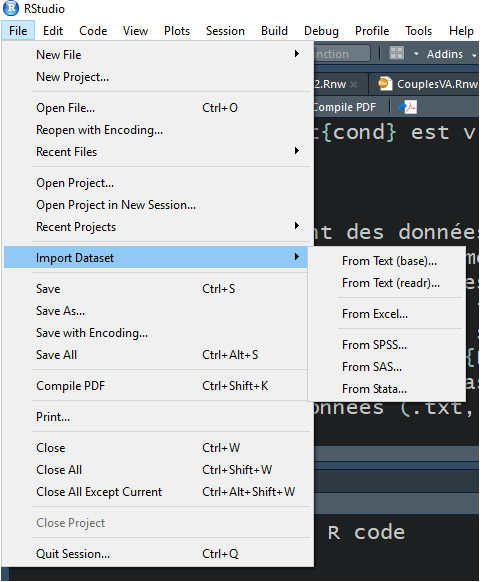
\includegraphics[width=0.75\linewidth,height=0.7\textheight]{impD} \end{center}
\end{frame}

\begin{frame}[fragile]{Saisir des données au clavier:}
\protect\hypertarget{saisir-des-donnuxe9es-au-clavier}{}
En utilisant la fonction \texttt{scan()}, la saisie d'une série de
données peut paraître moins fastidieuse.

\begin{Shaded}
\begin{Highlighting}[]
\NormalTok{jeu1}\OtherTok{=}\FunctionTok{scan}\NormalTok{()}
\DecValTok{1}\SpecialCharTok{:} \SpecialCharTok{{-}}\DecValTok{2}
\DecValTok{2}\SpecialCharTok{:} \DecValTok{1}
\DecValTok{3}\SpecialCharTok{:} \DecValTok{5}
\DecValTok{4}\SpecialCharTok{:} 
\NormalTok{jeu1}
\end{Highlighting}
\end{Shaded}

Le premier retour après une chaîne vide met fin à la saisie
\end{frame}

\begin{frame}[fragile]{Exporter une base de données:}
\protect\hypertarget{exporter-une-base-de-donnuxe9es}{}
Pour exporter un tableau de données, on fait appel à la fonction
\texttt{write.csv(x,\ file="",...)} où \texttt{x} est l'objet à exporter
et \texttt{file} est une chaîne de caractère précisant l'emplacement où
on veut enregistrer l'objet \texttt{x}.

\begin{Shaded}
\begin{Highlighting}[]
\NormalTok{xx}\OtherTok{=}\FunctionTok{matrix}\NormalTok{(}\FunctionTok{seq}\NormalTok{(}\DecValTok{0}\NormalTok{,}\DecValTok{5}\NormalTok{,}\AttributeTok{len=}\DecValTok{200}\NormalTok{),}\AttributeTok{nc=}\DecValTok{4}\NormalTok{)}
\FunctionTok{write.csv}\NormalTok{(xx, }\StringTok{"D:/Cours\_R/tab.csv"}\NormalTok{)}
\CommentTok{\# enregistrer l\textquotesingle{}objet xx dans le répertoire D:/Cours\_R }
\CommentTok{\# sous le nom tab avec l\textquotesingle{}extension .csv}
\end{Highlighting}
\end{Shaded}
\end{frame}

\end{document}
